\documentclass[11pt]{report}

\usepackage[T2A]{fontenc}
\usepackage[utf8x]{inputenc}
\usepackage[english, russian]{babel}

\usepackage[T1]{fontenc}
\usepackage{titlesec, blindtext, color}
\usepackage[left=3cm, right=3cm, bottom=4cm, top=3cm, bindingoffset=0cm]{geometry}

\usepackage{amsmath}
\usepackage{mathtext}
\usepackage{environ}

\usepackage{wrapfig}
\usepackage{graphicx}
\usepackage{caption}
\usepackage{subcaption}
\usepackage{tabularx}


\graphicspath{{img/}}

\definecolor{gray75}{gray}{0.75}
\newcommand{\hsp}{\hspace{20pt}}
\addto\captionsrussian{\renewcommand{\contentsname}{Содержание}}

\titleformat{\chapter}[hang]{\Huge\bfseries}{\thechapter\hsp\textcolor{gray75}{|}\hsp}{0pt}{\Huge\bfseries}


\newenvironment{itemize*}%
  {\begin{itemize}%
    \setlength{\itemsep}{2pt}%
    \setlength{\parskip}{0.75pt}}%
  {\end{itemize}}


\newenvironment{enumerate*}%
  {\begin{enumerate}%
    \setlength{\itemsep}{2pt}%
    \setlength{\parskip}{0.75pt}}%
  {\end{enumerate}}

\newcolumntype{R}{>{\rule{0pt}{0.55cm}\raggedleft\arraybackslash}X}%
\newcolumntype{L}{>{\rule{0pt}{0.55cm}\raggedright\arraybackslash}X}%
\newcolumntype{C}{>{\rule{0pt}{0.55cm}\centering\arraybackslash}X}%
\newcolumntype{P}{>{\rule{0pt}{0.55cm}\centering\hsize=\dimexpr2\hsize+2\tabcolsep+\arrayrulewidth\relax}X}%

\newenvironment{wrapfigure*}%
 {%
  \setlength{\columnsep}{15pt}%
  \wrapfloat{figure}}%
 {\endwrapfloat}


\NewEnviron{myequation}{%
\begin{equation}
\scalebox{1.5}{$\BODY$}
\end{equation}
}



\title{
	\textbf{Escapy2.0 Engine\\Specification and User Guide}
}
\author{Генрих Тимур Домагальски}
\date{31.07.2017 Издаине 1}



\begin{document}

\maketitle

\tableofcontents

\newpage

\chapter*{О движке}
Escapy2 это игровой движок написанный на java с использованием библиотек Dagger1, libGdx, box2d и Gson. Поскольку libGdx является лишь низкоуровневой оберткой над lwgjl - движок дает полноту простора в использовании openGL, в свою очередь Dagger делает код более модульным и масштабируемым.

\chapter{Начало работы}
Вход производится похожим образом как в libGDX и lwgjl - в main с созданием инстанции
\textbf{LwjglApplication}. Для этого создается объект \textbf{LwjglApplicationConfiguration} который загружается из json файла с помощью 
\textbf{EscapyDesktopConfigLoader}, о самих загрузчиках и механизме сериализации в движке более подробно потом. 

\begin{center}
	
\includegraphics[width=1.25\linewidth]{img/1.png} 
  	\label{img:1}
  	  	
  	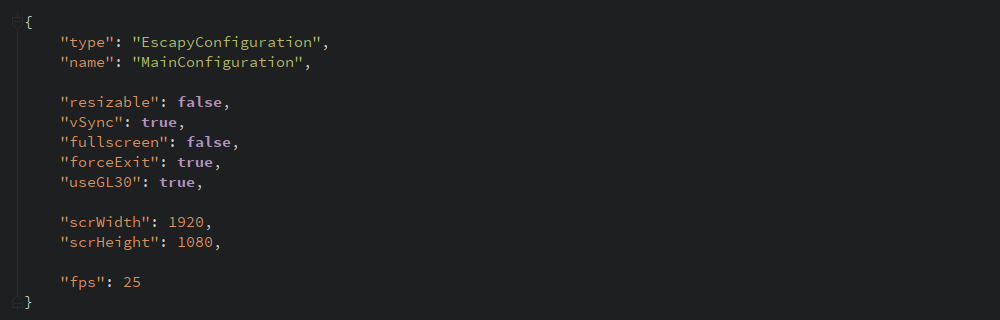
\includegraphics[width=1.25\linewidth]{img/2.png}   	
\end{center}
При создании \textbf{LwjglApplication} в качестве аргумента передается\\
\textbf{EscapyApplicationAdapter}, который в свою очередь в качестве аргумента принимает класс наследующийся от \textbf{EscapyGameContext} и varargs модулей Dagger'a.

\begin{center}
	
\includegraphics[width=1.25\linewidth]{img/3.png} 
  	\label{img:2} 
\end{center}
Подробнее о том как использовать модули Dagger'a можно прочитать на оффициальном  сайте проекта (\textit{http://square.github.io/dagger/}). \textbf{EscapyGameContext} имеет два конструктора, один из них как аргумент принимает инстанцию класса унаследованного от
\textbf{EscapyGameContextConfiguration} - абстрактного класса предоставляющего конфигурацию проекта через методы которые можно перегрузить в случае необходимости.




\end{document}




